% Chapter where we explain the results.

\chapter{Discussion}
\label{ch:discussion}

In this chapter we provide justifications for the choices made in solving the
protoboard layout problem, as well as detailed analysis of the data presented in
Chapter \ref{ch:results}.

\section{Search Space Size}
\label{sec:search_space_size}

The proposed solution to this problem involves several simplifications and uses
of heuristics. This is a result of the fact that the search space we are working
with is very large. It is difficult to say exactly how large this search space
is, but we can get an idea of its size. Let us just consider the number of ways
we can put down wires on an empty protoboard (even in ways that may not make
sense
from a circuit theoretic standpoint). Finding this number reduces to finding the
number of ways $T(n)$ in which we can choose pairs out of $n$ items. Equation
\ref{eq:telephone} givens an expression for $T(n)$\footnote{The sequence of
numbers described by $T(n)$ is sometimes referred to as the telephone numbers
or the involution numbers.}.

\begin{equation}
T(n) = \sum_{k = 0}^{\lfloor \frac{n}{2} \rfloor}{\frac{n!}{k! (n - 2k)! 2^k}}
\label{eq:telephone}
\end{equation}

In this problem, we have that $n = 830$, the number of available locations on an
empty protoboard. Evaluating $T$ at $n = 830$ yields approximately
$2.8\times10^{1043}$.
The largeness of this number indicates that doing any sort of exhaustive search
will be hopeless.

\section{Justifying Placement Choices}
\label{sec:justify_placement}

\subsubsection{Resistors}

For the sake of simplicity, and to significantly reduce the search space size, we
place resistors only in the middle strip of the protoboard, as shown in Figure
\ref{fig:piece_placement}. This choice is critical,
as the resistor pieces can generally be placed at numerous places on the
protoboard.
With this restriction, there are $63$ slots available for one resistor. Without
this restriction, there are a total of $763$ slots available. The restriction is
good when we consider the reduction in the search space size. On the other hand,
this restriction is bad as it imposes a restriction on the size of the
schematics (in terms of the number of components) for which a layout can be
generated using the algorithm.
Given that the number
of resistors in a typical 6.01 circuit is very
small, this restriction proves to be very useful.

\subsubsection{Op-amps}

Op-amps are the trickiest components to handle because each op-amp package put
on the protoboard contains two op-amps within it. Equation
\ref{eq:opamp} presents an expression for the number of
different ways to package together $n$ op-amps. For example, if we have $2$
op-amps, we can either use one op-amp package for each, or put them both in the
same package, which we can do in one of two different ways. All together, there
are $3$ different ways to package together $2$ op-amps\footnote{When using only
one of the op-amps in an op-amp package, we assume that we use the one on the
left as drawn in Figure \ref{fig:op_amp_pin_out}.}.
Table \ref{tb:opamp} gives the number of different packagings possible for
various $n$.

\begin{equation}
\text{Number of ways to package $n$ op-amps} =
\sum\limits_{k=0}^{\lfloor\frac{n}{2}\rfloor}{\frac{n!}{k!(n - 2k)!}}
\label{eq:opamp}
\end{equation}

\begin{table}
\begin{center}
\begin{singlespace}
\begin{tabular}{c | c}
$n$ & Number of ways to package $n$ op-amps \\
\hline
\hline
1 & 1 \\
2 & 3 \\
3 & 7 \\
4 & 25 \\
5 & 81 \\
6 & 331 \\
7 & 1303 \\
8 & 5937 \\
9 & 26785 \\
10 & 133651
\end{tabular}
\end{singlespace}
\end{center}
\caption[Op-amp packaging possibilities]{Number of ways of packaging together
$n$ op-amps for various values of $n$.}
\label{tb:opamp}
\end{table}

Our placement approach explores all possible ways
of packaging the op-amps. We do this because the typical 6.01 circuit contains
no more than $6$ op-amps, and so we are tasked with exploring at most $331$
alternatives, which is not too computationally intensive.
On circuits with more than $6$ op-amps, this approach quickly becomes
intractable, as the number of alternatives to consider would be
far too large, and we would have to consider different strategies.

\section{Explaining the Results}

Chapter \ref{ch:results} presented quantitative data to compare alternative
strategies for solving the protoboard layout problem. Here, we
analyze those data and give reasonings for why we obtained those results.

\subsection{Comparing Placement Methods}

\subsubsection{Success Rate}
The blocking placement method ($89.0\%$ overall success rate across the $44250$
runs)
is slightly more successful than the distance placement method ($87.6\%$ overall
success rate). While these alternative methods are not markedly different
in terms of success rate, we note that both methods are
more successful than the random placement alternative ($43.5\%$ overall success
rate).
As a function of circuit
complexity, Figure
\ref{fig:placement_success_trend} suggests that the two alternatives have almost
identical success rates. As we would expect, success rate generally decreases
for both of the placement methods as circuit complexity increases.
Once again, we observe that the distance and blocking based placement methods
are much more successful than the random placement method, especially as
circuit complexity increases.
The rise in success rate for high circuit complexity is a result of the fact
that there are very few circuits of the highest complexity, on which the
algorithm happened to be consistently successful.

\subsubsection{Wiring Time}
We observe from
Figure \ref{fig:placement_time_trend} that, once again, the two methods are
very similar, with random placement being markedly worse than both.
We see that the distance method generally results in a layout for which the
wiring takes less time than does the blocking method,
but the difference between the two is
almost negligible. As we would expect, we see that as the complexity
of the circuits increases, the amount of time spent in the wiring step also
increases. As circuit complexity increases, the standard error of
wiring time
when using random placement also increases. This is a result of
the fact that random placement frequently fails on the most complex
circuits, and so the sample size we have for successful runs is very small.

\subsubsection{Layout Quality}
Figure
\ref{fig:placement_quality_trend} presents graphs that compare numbers of wires,
numbers of wire crosses, and total wire lengths.
Figure \ref{fig:placement_badness_trend} shows the trend of layout badness
computed using our metric as a function of circuit complexity.
We first observe that the
number of wires used by the two methods are almost identical. We see that the
blocking method consistently results in more wire crosses. When we consider
total wire length, the blocking
method exceeds the distance method consistently, with the difference getting
higher as circuit complexity increases.
This is expected because the blocking method does not directly aim to
put pieces that need to be connected close together, whereas the distance method
directly tries to minimize the total wire length that may be needed. In terms
of the layout badness metric, we observe once again that the distance method
is slightly better than the blocking method for almost all circuit complexity
values. Finally, we observe that the random
placement method, per our badness metric, produces much worse layouts than the
other two methods when it does succeed.

\subsubsection{Conclusion}
It is difficult to conclusively pick the best placement method from these
results. What we can determine is that the distance based method and the
blocking based method are both better than random placement.

\subsection{Comparing Wiring Methods}

\subsubsection{Success Rate}
Figures \ref{fig:wiring_success} and \ref{fig:wiring_success_trend}, and Table
\ref{tb:wiring_success} show that the all pairs wiring method has a much smaller
success rate than all of
the other alternatives, especially as circuit complexity increases. The reason
why the all pairs method has a smaller success rate is in
large part due to the limit on expanded vertices in $A*$.
Figure \ref{fig:max_expanded} depicts histograms of the maximum number of
states expanded in a search for each of the $4425 \times 10 = 44250$ test runs.
In the case of all pairs wiring, the histogram is simply of the number of
states expanded in the search for each of the test runs. In the other methods,
multiple searches may be carried out per run, and we chose to look at the most
expensive search in our analysis to understand the worst-case performance of
the alternative methods. The figures depict that the limit on expanded
vertices affects
the all pairs wiring method much more than it does the others. This result is
expected because the search task in all pairs wiring is more difficult than in
the other alternatives. Notice that as the search tasks get less difficult from
all pairs to per-node to per-pair wiring, the effect of the limit
decreases. Hence, the other four alternatives have very comparable success rates.
Finally, we note that straight wiring, as expected, has a $100\%$ success rate.

\begin{figure}[H]
\begin{center}
\subfigure[All pairs]{
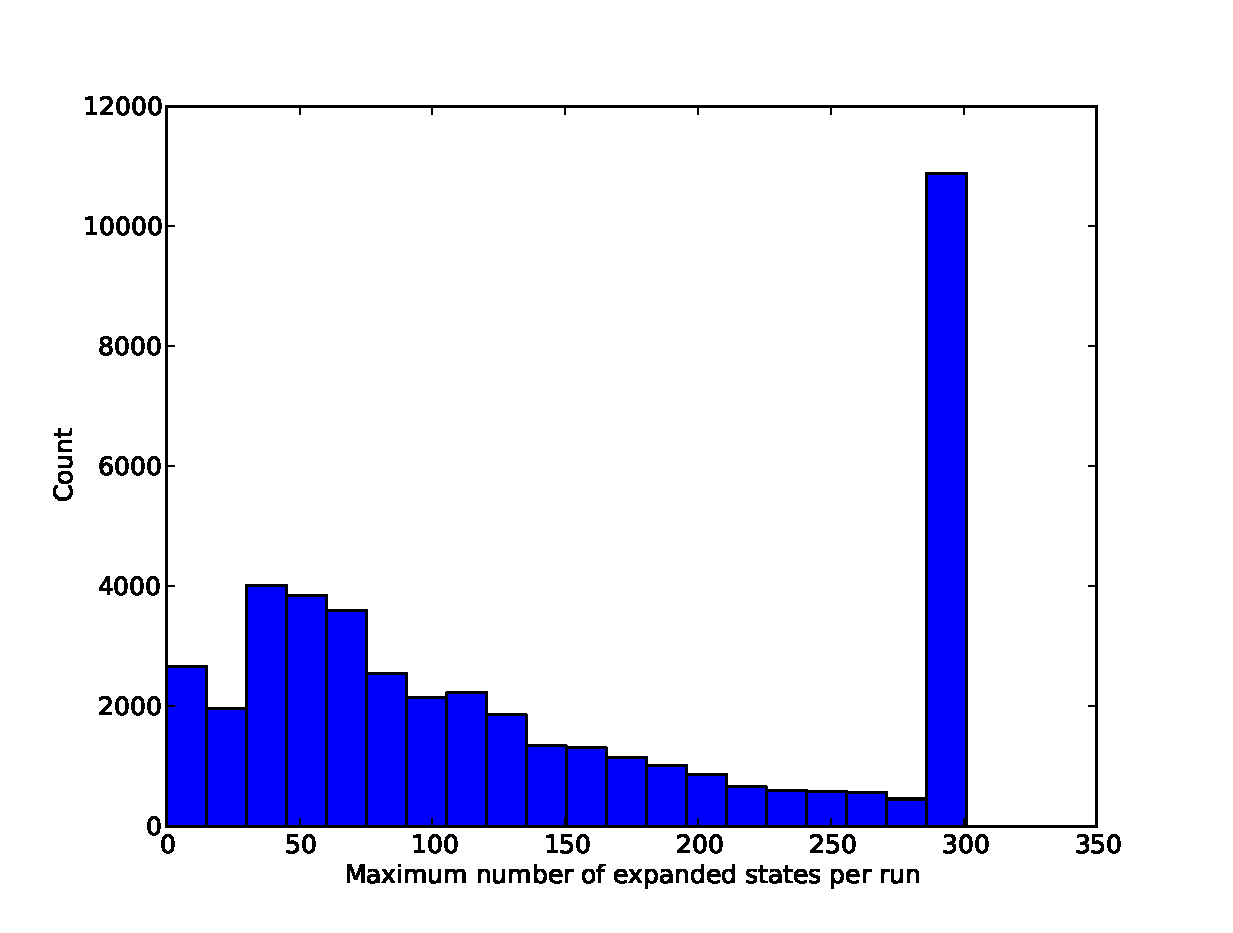
\includegraphics[width=7cm]{Images/max_expanded_all_pairs.eps}}\\
\subfigure[Per node (increasing)]{
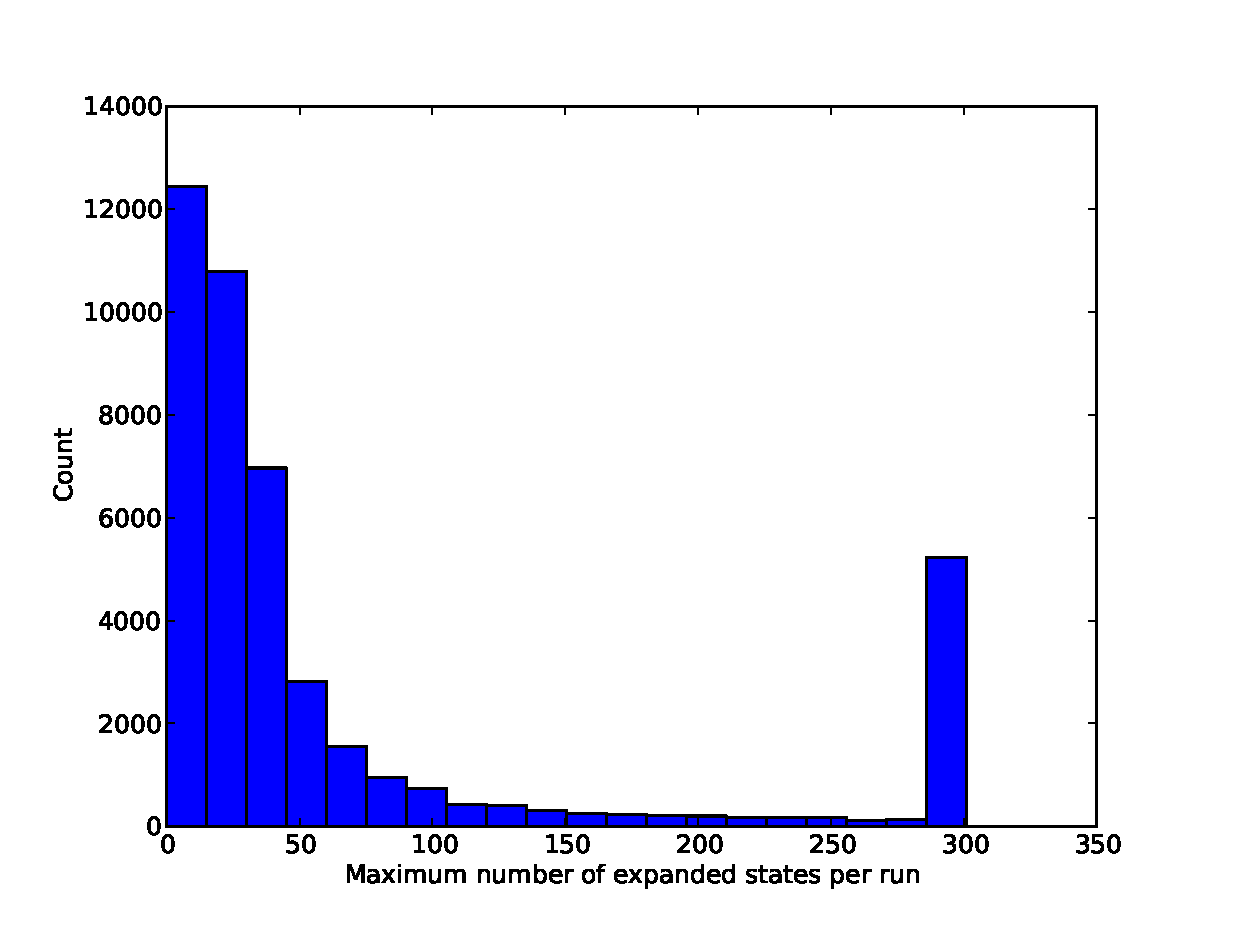
\includegraphics[width=7cm]{Images/max_expanded_per_node_increasing.eps}}
\subfigure[Per node (decreasing)]{
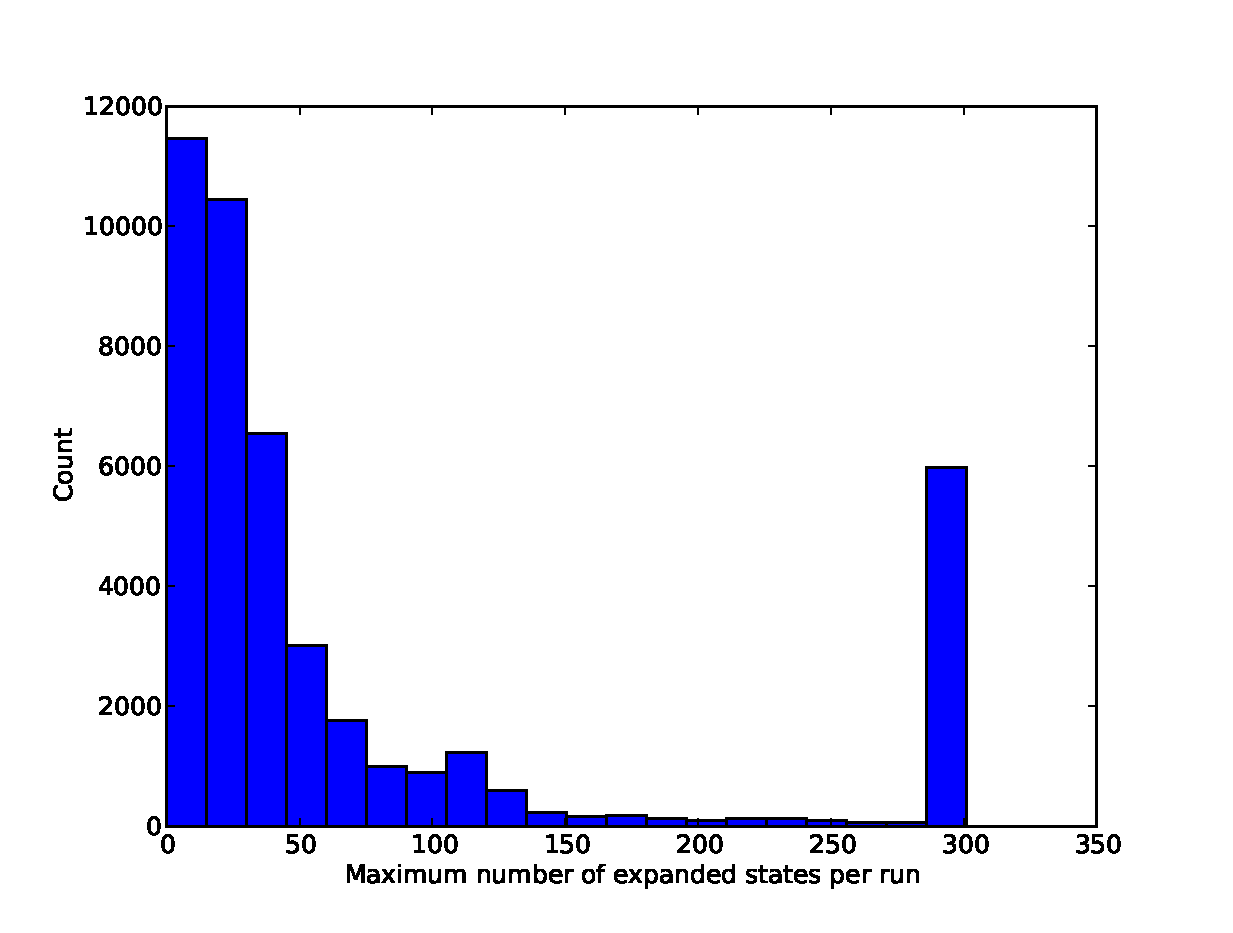
\includegraphics[width=7cm]{Images/max_expanded_per_node_decreasing.eps}}
\subfigure[Per pair (increasing)]{
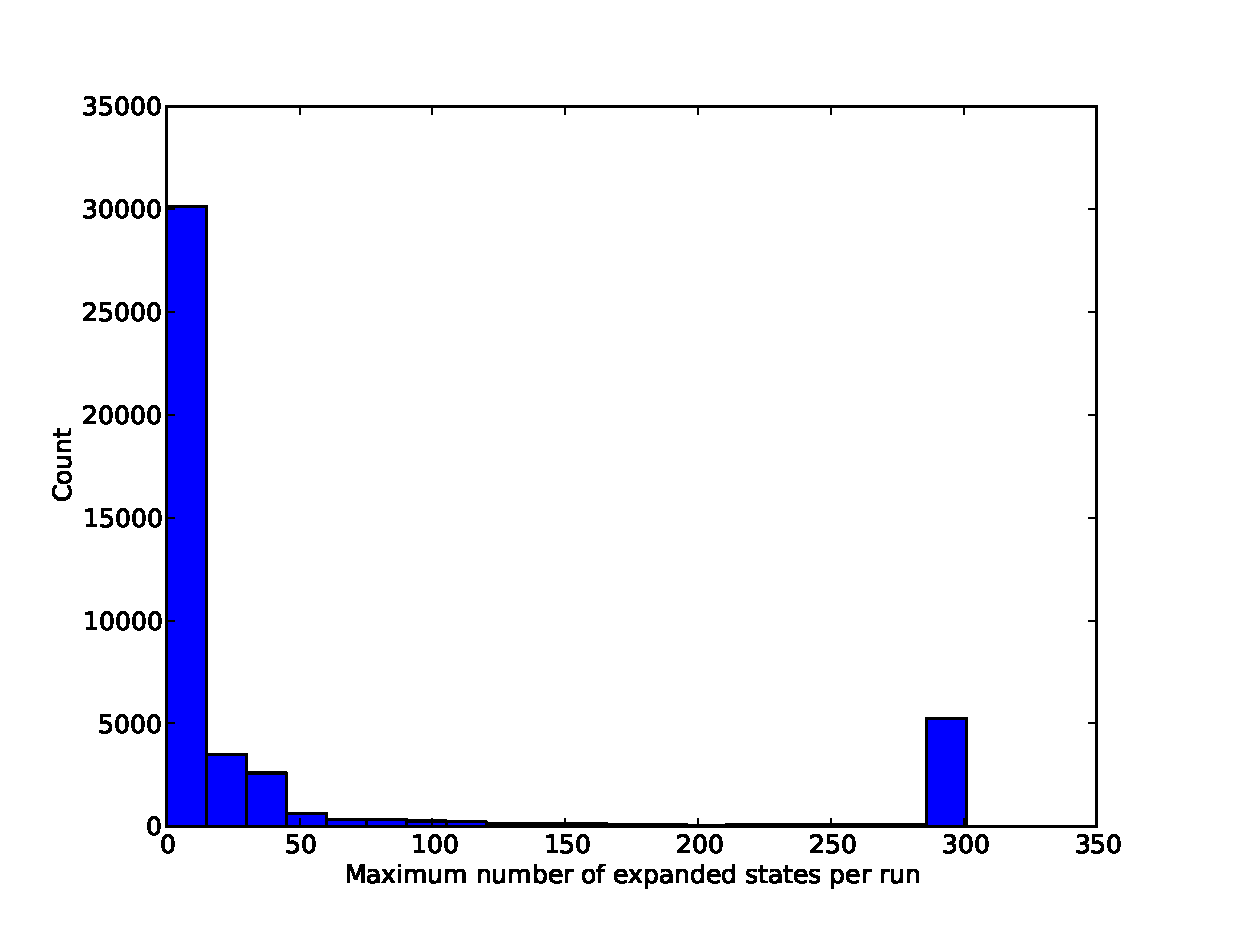
\includegraphics[width=7cm]{Images/max_expanded_per_pair_increasing.eps}}
\subfigure[Per pair (decreasing)]{
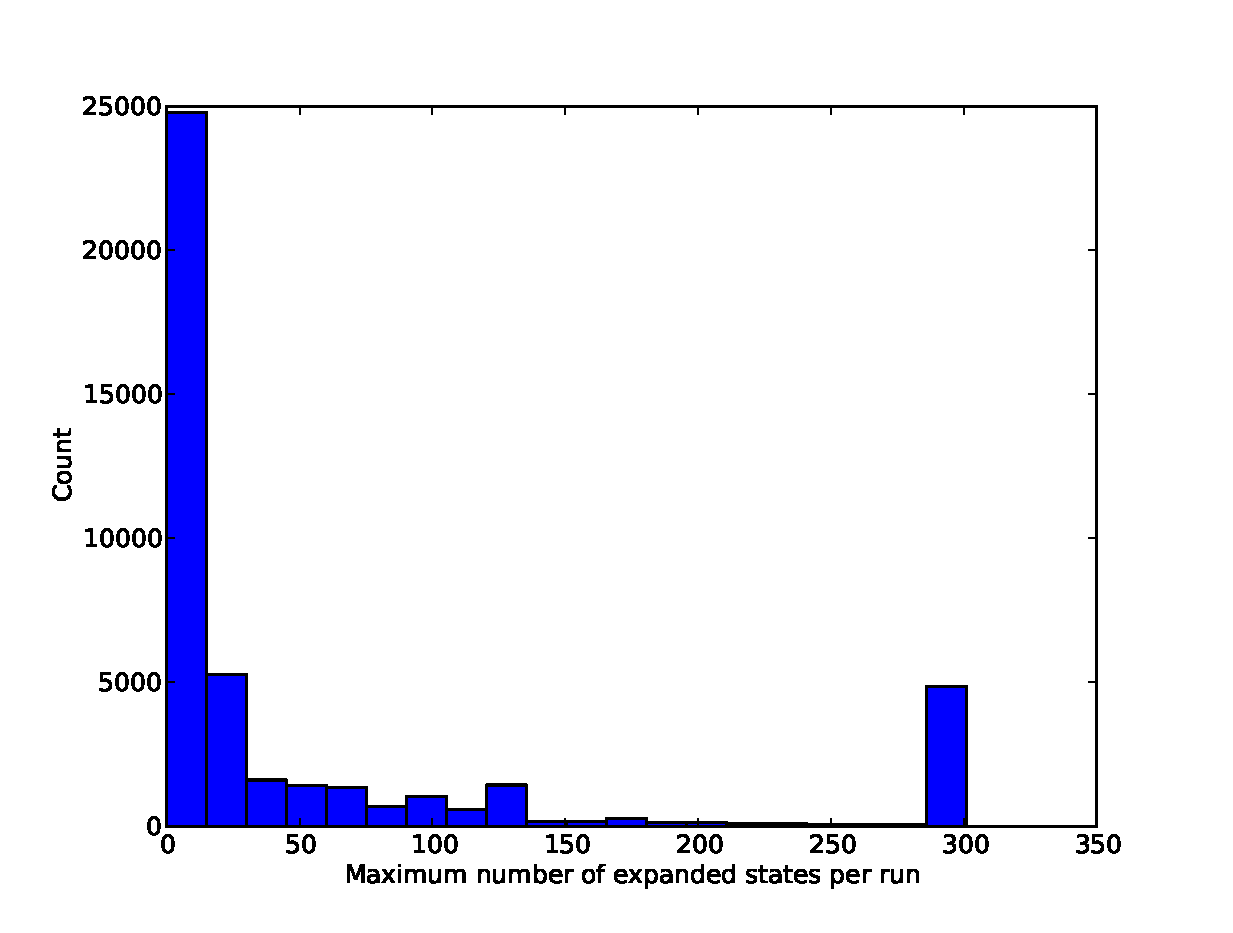
\includegraphics[width=7cm]{Images/max_expanded_per_pair_decreasing.eps}}
\caption[Expanded vertices histograms]{Histograms of maximum number of vertices
expanded in $A*$ per test run.
In the case of all pairs wiring, this value is simply the number of vertices
expanded in the search.}
\label{fig:max_expanded}
\end{center}
\end{figure}

\subsubsection{Wiring Time}
Figure \ref{fig:wiring_time_trend} compares wiring time across
the six methods. Once again, we observe that the all pairs methods takes
more time than the other methods. We also observe from Figure
\ref{fig:wiring_time_trend} that the wiring times for the two per-node methods
are comparable, and that the wiring times for the two per-pair methods are also
comparable, but that the per-node wiring times are generally bigger than the
per-pair wiring times. This trend is also expected as the per-node methods
attempt to connect multiple pairs of locations at once, which generally requires
searching through more alternatives than
connecting each of the pairs of locations individually.
Finally, we note that straight wiring, as expected, takes less time to complete
than all of the other alternatives.

\subsubsection{Layout Quality}
Figures \ref{fig:wiring_quality_trend} and
\ref{fig:wiring_badness_trend} compare the
quality of the layouts produced by the six alternative wiring methods. First,
as we observed in the placement method comparison, we see that there is very
little difference in terms of number of wires used and the total wire length
among the alternatives that utilize search to accomplish the wiring. We note
that straight wiring uses uses fewer wires than all of the other alternatives
as it uses exactly one wire per pair of locations.
There are noticeable differences in the number of wire crosses. We see
that the all pairs method generates layouts with much fewer wire crosses than
the other methods. This is expected since the algorithm runs one search to
connect all pairs of locations. Conversely, the per-pair (decreasing) and
per-node (decreasing) methods
result in the largest number of wire crosses. Note that
the per-node (decreasing) method produces more wire crosses on average than the
per-pair (increasing) method.
We observe that the order in which we consider pairs of
locations has an effect on how good the generated layouts will be.
In essence, connecting the harder pairs of locations first generally produces
more wire crosses.
Finally, as expected, we observe that straight wiring produces comparatively
poor layouts.

\subsubsection{Conclusion}
While the all pairs method is the least successful
method and generally takes the longest among the six,
it tends to produce the best layouts when it does succeed. On the other hand,
the alternatives that break the problem down into smaller pieces succeed more
often and finish more quickly, though they tend to produce worse results.
Furthermore,
the more finely we break down the problem, the faster the overall algorithm runs.
Lastly, ordering subproblems from hardest to easiest has the effect of making the
overall wiring step faster, but produces worse results than the reverse
order and does not result in a markedly better success rate.

\subsection{Comparing Search Methods}

\subsubsection{Success Rate}
Figures \ref{fig:search_success} and
\ref{fig:search_success_trend} and Table \ref{tb:search_success} present
data comparing the success rates of the two search algorithms.
We observe that Best First Search is much more
successful than $A*$. $98\%$ of the test circuits were solved at least $8$ times
out of $10$ when we used Best First Search, versus $85\%$ when we used $A*$.
This result is not surprising because, when using Best First Search,
the algorithm
looks for layouts that satisfy the connection requirements, ignoring the badness
of the layouts it considers, whereas $A*$ searches for an ``optimal'' layout.
Hence, Best First Search is less susceptible to the
restriction on number of vertices to expand than is $A*$.

\subsubsection{Wiring Time}
The fact that Best First Search settles for any layout that satisfies the
connection
requirements suggests that it should finish more quickly in addition to being
more successful. Figure \ref{fig:search_time_trend} supports this
expectation.

\subsubsection{Layout Quality}
Figures \ref{fig:search_quality_trend} and \ref{fig:search_badness_trend} show
that the layouts generated by the
algorithm when using Best First Search are worse than the layouts generated
when using $A*$. Most importantly, the
number of wire crosses in the layouts produced by Best First Search are markedly
greater than the number of wire crosses in the layouts produced by $A*$. We also
observe that the total wire length is greater when using Best First Search.

\subsubsection{Conclusion}
Our choice of a search algorithm forces us to consider a trade-off between
speed, success rate, and quality.
Using Best First Search, most runs will be successful
and terminate quickly, but will produce very poor results. Using $A*$,
fewer runs will be successful, and the successful runs will take longer to
terminate, but the resulting layouts will generally be better.

\subsection{Combined Algorithm}
\label{sec:method_combination}

In this section we discuss the structure of Algorithm
\ref{alg:combined}, and we also
discuss the data we obtained for the combined algorithm. Recall that the combined
algorithm makes four attempts at generating a complete layout. The algorithm
tries both
placement methods, using the distance method first and the blocking method
second. It
tries the distance method first because the distance method tends to
generate layouts with fewer
crossing wires and smaller total wire length. The algorithm uses
per-pair wiring, and
consider both orders of doing the wiring, increasing order first and decreasing
order second. It uses per-pair wiring because per-pair wiring takes considerably
less time than both per-node and all pairs wiring, and neither of the other
wiring methods has a better success rate. The algorithm tries increasing order
first because increasing order tends to generate layouts with fewer crossing
wires than the reverse order.

Let us now consider the data we obtained for the combined algorithm. Firstly, we
see that the combined algorithm had a $100\%$ success rate, which is critical
when we consider the fact that students will be using a tool that almost never
fails. This success rate is a result of the last part of Algorithm
\ref{alg:combined} that uses single wires to connect pairs of locations that
need to be connected.
Figure \ref{fig:final_num_trials} shows that, on the test dataset of $4425$
schematics, with $10$ runs carried out on each schematic, the algorithm succeeded
in generating layouts for $98.6\%$ of the circuits without having to put down
forced wires (wires added at the last step of the algorithm to connect any
disconnected location pairs). The algorithm was
required to put down more than $2$ forced wires on only $0.1\%$ of the circuits.
From Figure
\ref{fig:final_time_trend}, we see that as the circuit gets more complex, the
amount of time the algorithm takes sharply increases. This is due to a more
difficult placement task (which is most notable as the number of op-amps
increases) as well as a more
difficult wiring task. Importantly, the maximum
point on the plot occurs at less than $180$ seconds. This indicates that on the
test dataset, the algorithm took at most about $3$ minutes to run. This is
encouraging from a practical standpoint because $3$ minutes is not long
for a student to have to wait for a layout to be generated.
Finally, Figures \ref{fig:final_quality_trend} and \ref{fig:final_badness_trend}
present trends of quality as a
function of circuit complexity.

\section{Further Work}

\subsection{Treating Resistors as Wires}

Our current solution treats resistors as circuit components and so they are
placed before the wiring search is executed.
However, resistors have the special property among the components that
they can be placed as if they were wires of a fixed set of lengths.
This suggests we can think of resistors as wires,
and thus can handle them in the wiring step of the algorithm instead of
the placement step. As a result, the search that we do in the wiring step would
need to be
more elaborate. Not only would we need to keep track of pairs of locations on the
protoboard that need to be connected, but we would also need to know whether to
put a resistor between the two locations. In the latter case, we have the
restriction that one of the wires we use to connect the pair of locations needs
to be of a length that can fit a resistor.

While this idea appears very promising, its implementation is not trivial.
First, if there is any node in the circuit that is only
connected to resistors (and no other circuit components), then that node will be
unrepresented on the protoboard at the end of the placement step. One possible
solution to this problem is to reserve an empty column on the
protoboard for the node between the resistors, which we can then use in the
wiring step. A better solution may
be discovering the best places for the node as we are placing down resistors in
the wiring step, but this solution would make the search we carry out
more complicated. Second, we would need a new kind of heuristic for the
search that takes resistors into account. One possible solution is to highly
penalize an absent resistor when computing the heuristic.
Even with an amended heuristic, however, there
are cases where the search may not find an answer (for instance a pair of
adjacent locations that must be connected by a resistor).

\subsection{Building Layouts Similar to Previously Generated Layouts}
One problem with the current tool is that a slight change in
the circuit schematic may result in a completely different layout. It is,
therefore, very important that students in 6.01 be confident that they designed
the right circuit before taking the time to build their circuit.
This is where the simulation
capabilities of the tool come in to play. As an alternative solution to this
problem, it may be useful to have the
tool remember the last placement it used and try to produce a new placement as
similar to the last one as possible.

\section{Remarks}

This paper introduced a circuit schematic entry tool for 6.01 capable of
automatically generating protoboard layouts. The final algorithm presented in
this paper is able to generate layouts with a $100\%$ success rate on our test
dataset, and produces markedly better layouts than randomly generated ones based
on our metric of layout badness. These results are encouraging as they suggest
that the tool may be a good addition to 6.01 as a compliment, or perhaps
replacement, for CMax. If, as
we intended, the tool's performance on the test schematics is any indication of
its performance on schematics that 6.01 students may design, then the tool
achieves the goal of avoiding the tedium of protoboard layout in 6.01 labs.
Additionally, the schematic entry tool, which is also capable of circuit
analysis at the same level as CMax, would make circuits schematics the main
mode of communication in 6.01 labs (instead of protoboard layouts).
